\let\negmedspace\undefined
\let\negthickspace\undefined
\documentclass[journal,12pt,onecolumn]{IEEEtran}
\usepackage{cite}
\usepackage{amsmath,amssymb,amsfonts,amsthm}
\usepackage{algorithmic}
\usepackage{graphicx}
\usepackage{textcomp}
\usepackage{xcolor}
\usepackage{txfonts}
\usepackage{listings}
\usepackage{enumitem}
\usepackage{mathtools}
\usepackage{gensymb}
\usepackage[breaklinks=true]{hyperref}
\usepackage{tkz-euclide} % loads  TikZ and tkz-base
\usepackage{listings}
\usepackage{gvv}
\usepackage{circuitikz}

\newtheorem{theorem}{Theorem}[section]
\newtheorem{problem}{Problem}
\newtheorem{proposition}{Proposition}[section]
\newtheorem{lemma}{Lemma}[section]
\newtheorem{corollary}[theorem]{Corollary}
\newtheorem{example}{Example}[section]
\newtheorem{definition}[problem]{Definition}

\newcommand{\BEQA}{\begin{eqnarray}}
\newcommand{\EEQA}{\end{eqnarray}}
\newcommand{\define}{\stackrel{\triangle}{=}}
\theoremstyle{remark}
\newtheorem{rem}{Remark}

\graphicspath{./figs/}

%\bibliographystyle{ieeetr}
\begin{document}
%

\bibliographystyle{IEEEtran}


\vspace{3cm}

\title{
	%	\logo{
	Gate Assignment

	\large{EE:1205 Signals and Systems}

	Indian Institute of Technology, Hyderabad
	%	}
}
\author{Kunal Thorawade

EE23BTECH11035
}	
\maketitle


%\tableofcontents

\bigskip
 
 \renewcommand{\thefigure}{\theenumi}
 \renewcommand{\thetable}{\arabic{table}}
 \renewcommand{\thefigure}{\arabic{figure}}
 %\renewcommand{\theequation}{\theenumi}

 \textbf{Question}:
 A Spectrometer is used to detect plasma oscillations in a sample. The spectrometer 
 can work in the range of $3 \times 10^{12}$ rad s$^{-1}$ to $30 \times 10^{12}$ rad s$^{-1}$. The minimum carrier concentration that can be detected by using this spectrometer is $n \times 10^{21}$ m$^{-3}$. The value of $n$ is \underline{\hspace{2cm}}. (Round off to two places)
 (Charge on electron $= -1.6 \times 10^{-19} $ C$^{-1}$, mass of electron = $9.1 \times 10^{-31}$ kg and $\epsilon_0 = 8.85 \times 10^{-12}$ C$^{2}$ N$^{-1}$ m$^{-2}$ ) \hfill(GATE PH 35 2022)\\
 \solution 
 \begin{table}[ht]
  \centering
    \begin{tabular}{|c|c|}
        \hline
	   \textbf{ Parameter} & \textbf{Description} \\
	        \hline
		     $\rho_1$ & Density of Liquid \\
		          \hline
			       $\rho$ & Density of cork \\
			            \hline
				         $h$ & Height of cylindrical cork \\
					      \hline
					           $x$ & Displacement \\
						        \hline
							    $T$ & Time period \\
							        \hline
								    $A$ & Base area of cylindrical cork \\
								        \hline
									    $F_R$ & Restoring Force \\
									        \hline
										    $a$ & Acceleration \\
										        \hline
											    $\omega$ & Angular Frequency \\
											        \hline
												    $m = \rho Ah$ & Mass of cylindrical cork \\
												        \hline
													  \end{tabular}
													    \vspace{2mm}
													      \caption{Parameter Table}
													        \label{11.14.18}
														\end{table}

 \begin{align}
	     \Delta\omega_p &= \sqrt{\frac{n_0e^2}{m\epsilon_0}} \\
	         \implies n_0 &= \frac{\brak{\Delta\omega_p}^2m\epsilon_0}{e^2} \\
		     n_0 &= \frac{\brak{27 \times 10^{12}}^2 \times \brak{9.1 \times 10^{31} }\times \brak{8.85 \times 10^{-12}}}{\brak{-1.6 \times 10^{-19}}^2} \\
		         \therefore n_0 &= 2.83 \times 10^{21} \text{m}^{-3} \\
			     n &= n_0 \times 10^{-21} \\
			         \therefore n &= 2.83
 \end{align}
 \begin{figure}[ht]
	     \centering
	         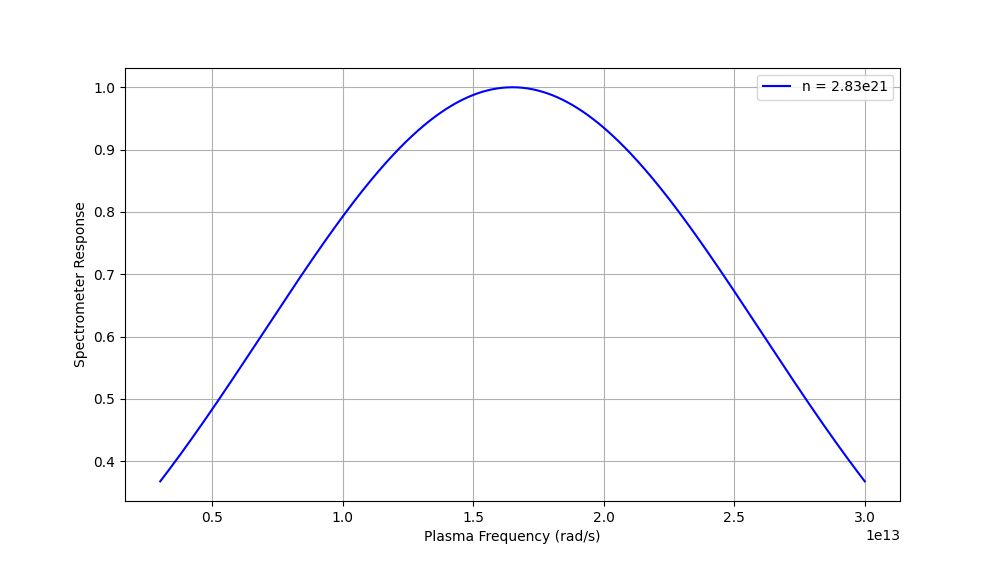
\includegraphics[width = \columnwidth]{figs/fig1.jpg}
		     \caption{Plot of Spectrometer response vs Plasma frequency}
		         \label{fig2.PH.35}
 \end{figure}
\end{document}
